\documentclass[aspectratio=169]{beamer}
\usepackage{will_handley_beamer}
\usepackage{title_page}
\usepackage{slashed}

% Commands
% --------
% - \arxiv{arxiv number}
% - \cols{width}{lh column}{rh column}
% -  \begin{fig(left|right)}[fractional width (e.g 0.6) ]{name of image}
%        content of other column
%    \end{fig(left|right)}

% Talk details
% ------------
\title{Resonant or asymmetric: The status of sub-GeV dark matter }
\subtitle{\arxiv{2405.17548}}
\date{21\textsuperscript{st} June 2024}

\begin{document}

\begin{frame}
    \titlepage
\end{frame}

\begin{frame}
    \frametitle{<+Frame title+>}
    <+Content+>

    Slide indicating all the components going into this fit
    \arxiv{2405.17548}
\end{frame}

\begin{frame}
    \frametitle{Physics}
    \begin{itemize}
        \item Dark photon $A'$ with mass $\boxed{m_{A'}}$ (via Stueckelberg mechanism) with kinetic mixing $\boxed{\kappa}$.
            \[\mathcal{L} = -\frac{1}{2}m_{A'}^2 A'_\mu A'^\mu - \frac{1}{4}A'_{\mu\nu}A'^{\mu\nu} - \kappa e A'^\mu \sum_{f\in\text{SM}} q_f \bar f \gamma_\mu f\]
        \item Dark matter candidate $\chi$ with mass $\boxed{m_\text{DM}}$, with $\chi\in\{\Phi, \psi\}$ complex scalar or Dirac fermion, coupled to the dark photon with $\boxed{g_\text{DM}}$.
        \begin{align*}
            \mathcal{L}_\psi  =& \bar{\psi}(i \slashed{\partial} - m_\text{DM}) \psi + g_\text{DM} A'^\mu \bar{\psi} \gamma_\mu \psi \\
            \mathcal{L}_\Phi  =& |\partial_\mu \Phi|^2 - m_\text{DM}^2 |\Phi|^2 - g_\text{DM}^2 A'_\mu A'^\mu |\Phi|^2 + i g_\text{DM} A'^\mu \left[\Phi^\ast (\partial_\mu \Phi) - (\partial_\mu \Phi^\ast) \Phi\right],
        \end{align*}
    \item Dark matter different from its anti-particle, there may be an asymmetry $\boxed{\eta_\text{DM}}$
    \item Also have local halo DM density $\rho_0$, velocity dispersion $v_0$ and escape velocity $v_\text{esc}$ as nuisance parameters determined by Gaia data~\arxiv{1901.02016} \textit{et al}.
    \item Focus on sub GeV region $\text{MeV} < m_\text{DM} < \text{GeV}$.
    \end{itemize}
\end{frame}

\begin{frame}
    \frametitle{Data}
    \begin{columns}
        \column{0.5\textwidth}
        \begin{block}{Cosmological constraints}
                CMB \& BBN

            $\Omega_c h^2 \approx 0.120\pm0.001$ from \textit{Planck}

            $N_\text{eff}\approx 2.99\pm 0.17$ via \texttt{AlterBBN}
            %Exotic energy injections $p_\text{ann}$ affect recombination
        \end{block}
        \begin{block}{Astrophysical constraints}
            X-rays \& Bullet cluster

            MeV gap (INTEGRAL is sub-MeV, Fermi-LAT is super-GeV)

            INTEGRAL, NuStar, XMM-Newton, Suzaku

            secondary signals odf DM annihilation (inverse compton scattering of products producing keV XRays


                Bullet cluster gives self-interaction constraints, since interactions make friction, and would cause subcluster to lose DM. (focus on the latter due to need for SBI for the former).
        \end{block}
        \column{0.5\textwidth}
        \begin{block}{Accelerator constraints}
            Beam dumps \& electron-positron colliders

            dark photon decays into pairs of DM particles

            constraints come from 'missing energy searches' 

            (beam dump): LSND, MiniBooNE
            'missing energy searches': NA64, BaBar

            also 
        \end{block}
        \begin{block}{Direct detection constraints}
            searches for electron \& nuclear recoils

            Xenon1T, SENSEI, DarkSide50, PandaX-4T, DAMIC-M SuperCDMS HV
        \end{block}
        <++>
    \end{columns}
\end{frame}

\begin{frame}
    \frametitle{GAMBIT}
\end{frame}

\begin{frame}
    \frametitle{Parameter estimation}
\end{frame}

\begin{frame}
    \frametitle{Model comparison}
\end{frame}

\begin{frame}
    \frametitle{Further work}
\end{frame}

\begin{frame}
    \frametitle{Conclusions}
    \framesubtitle{\tthref{github.com/handley-lab}}
    \tikz[overlay,remember picture]
        \node[anchor=north east] (A) at ($(current page.north east)+(0,0)$) {
            
\includegraphics[width=0.09\textheight]{figures/students/adam_ormondroyd.jpg}%
            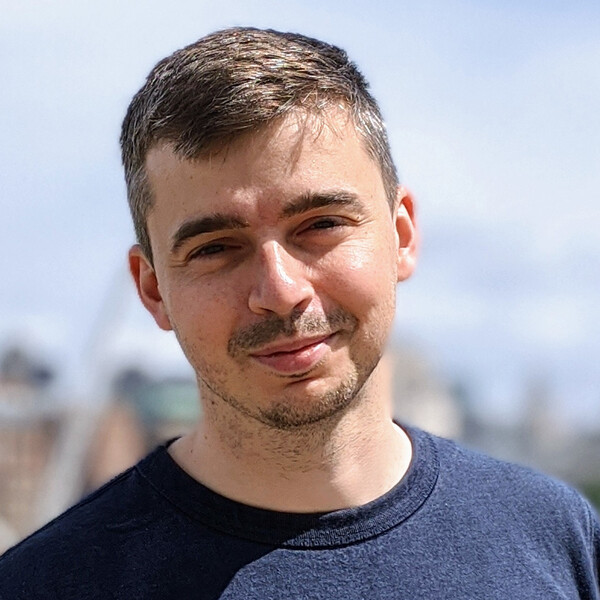
\includegraphics[width=0.09\textheight]{figures/students/david_yallup.jpg}%
            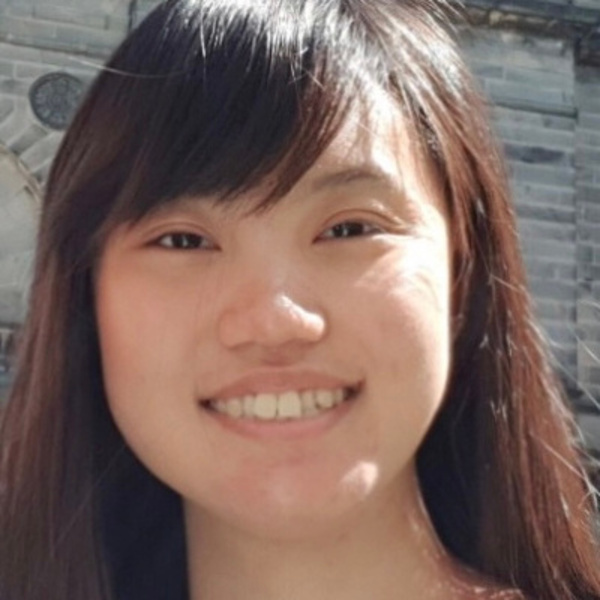
\includegraphics[width=0.09\textheight]{figures/students/dily_ong.jpg}%
            
\includegraphics[width=0.09\textheight]{figures/students/felicity_ibrahim.jpg}%
            
\includegraphics[width=0.09\textheight]{figures/students/george_carter.jpg}%
            
\includegraphics[width=0.09\textheight]{figures/students/harry_bevins.jpg}%
            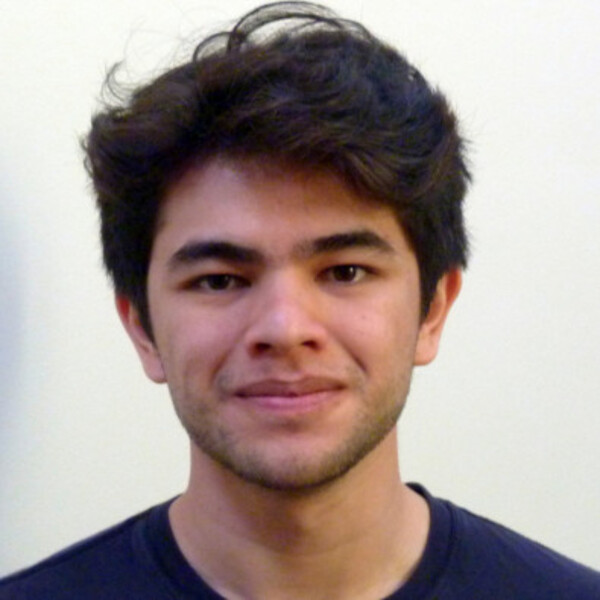
\includegraphics[width=0.09\textheight]{figures/students/ian_roque.jpg}%
            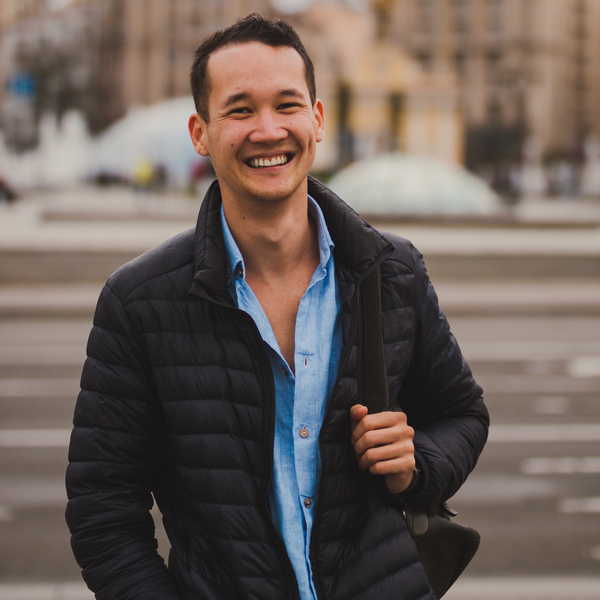
\includegraphics[width=0.09\textheight]{figures/students/kilian_scheutwinkel.jpg}%
            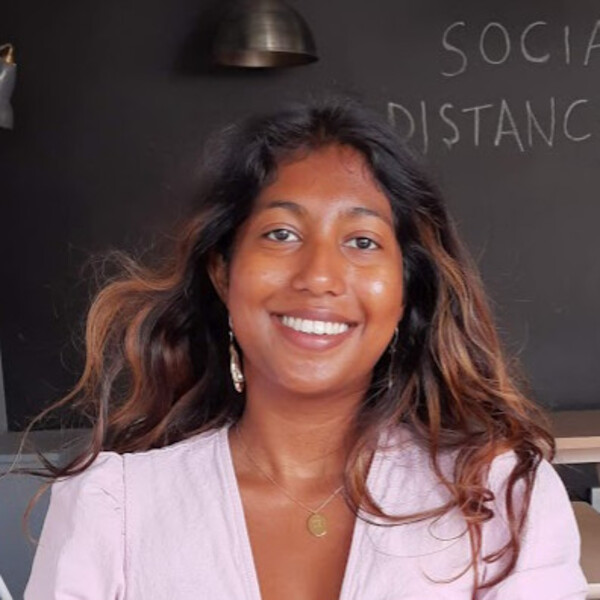
\includegraphics[width=0.09\textheight]{figures/students/metha_prathaban.jpg}%
            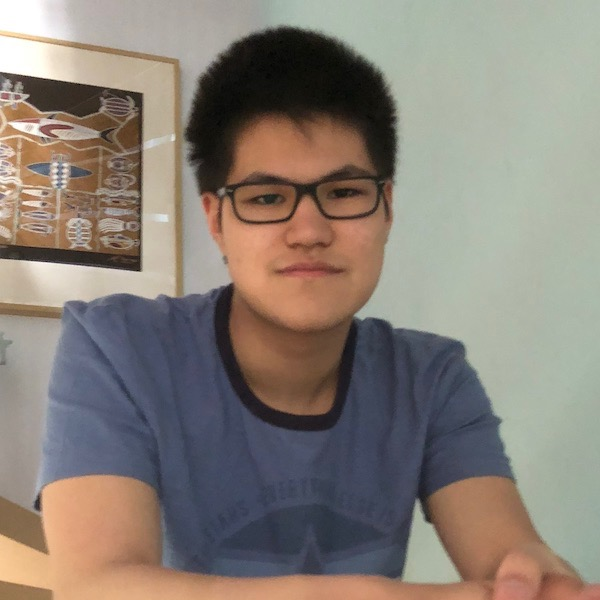
\includegraphics[width=0.09\textheight]{figures/students/namu_kroupa.jpg}%
            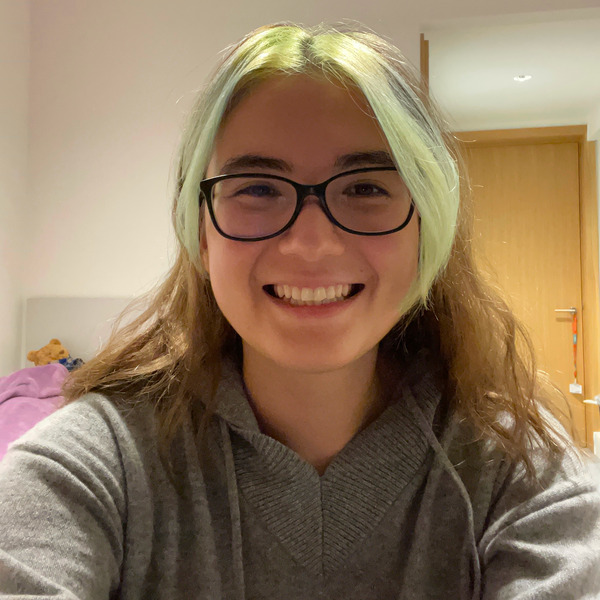
\includegraphics[width=0.09\textheight]{figures/students/sinah_legner.jpg}%
            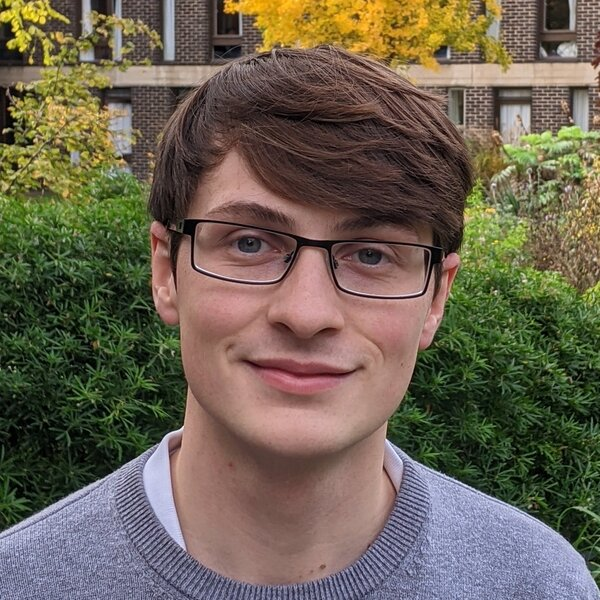
\includegraphics[width=0.09\textheight]{figures/students/thomas_gessey-jones.jpg}%
            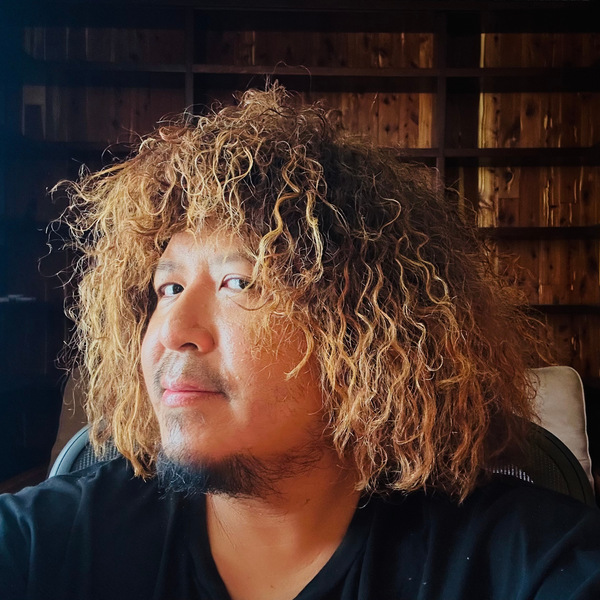
\includegraphics[width=0.09\textheight]{figures/students/tze_goh.jpg}%
            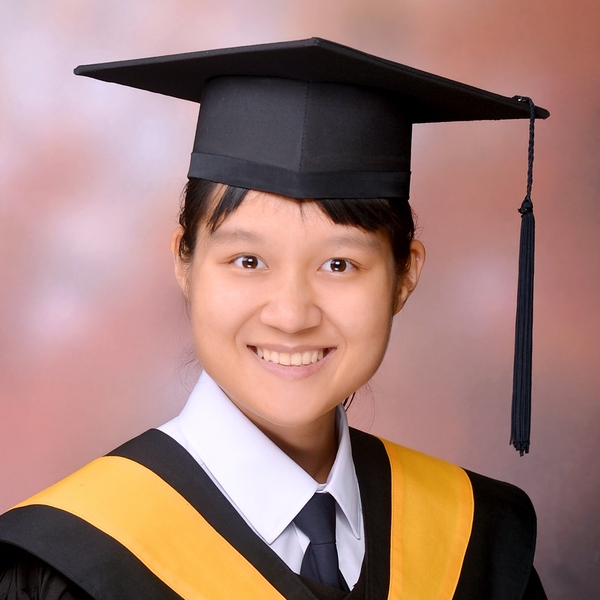
\includegraphics[width=0.09\textheight]{figures/students/wei-ning_deng.jpg}%
    };
\end{frame}

\end{document}
